\documentclass[12pt]{beamer}
\usetheme{UMNGolphers}




\title{\LARGE Asymptotic Limit Setting in CMS}
%\vskip400pt
%\subtitle{ UMN Meeting}
\author{Tambe E. Norbert}
\date{\today}
%\institute{\url{norbert@physics.umn.edu}\\\url{http://www.physics.umn.edu/people/norbert.html}}
%\institute{ University of Minnesota,\\ \url{norbert@physics.umn.edu}}
\institute{ \url{norbert@physics.umn.edu}}


\begin{document}
% Align Titile in center
\begin{frame}[c]
\titlepage
\end{frame}
\section{Motivation}
\begin{frame}
\Large
\frametitle{Outline}
\tableofcontents
\end{frame}

\section*{Motivation}
\begin{frame}
\frametitle{Motivation}
%\vspace{-1cm}
\begin{itemize}
\Large{
\item <1-| alert@1> Quick computation of limits. 
%\item <1-| alert@1> Quick access to limits without need for resourceful Monte Carlo Computation.
\item  Study systematic effects.
%\item  Study the effects of uncertainties in a given measurement.
\item Extract experiment sensitivity with ease.
%\item Easy approach to characterise the sensitivity of an experiment through the expected significance
\item  Quantify statistical significance of a signal.
%\item  Quantify statistical significance of an observed signal.
%\item Hypothesis Testing.
%\item Computing the confidence interval or upper limit of a given parameter
}
\end{itemize}
\begin{block}{Hypothesis Compatibility with Data?}

\end{block}
\end{frame}

\section{Statistical Formalism}
\begin{frame}
\frametitle{CLs Technique}
\begin{block}{Past Week}
\begin{enumerate}
%\item Limit setting: Have been working on limit setting using standard CMS tool.
\item GMSB/GGM MC samples for final limit setting
\item Limit setting with systematics.
\item Making standard CMS style plots. 
\item Writing Thesis
\end{enumerate}
\end{block}

\begin{block}{Plans}
\begin{enumerate}
\item Producing MC samples for GGM
\item Limit  with HybridNew Setting.
\item Make Analysis slides/Writing Thesis.
\item Update Analysis note with new plots.

\end{enumerate}

\end{block}
\end{frame}


\section{Test Statistics}
\begin{frame}
\frametitle{Test Statistics Distribution}
\vspace{-4cm}
Finding significance involves Monte Carlo calculations $\Rightarrow$ computationally expensive.
\subsection{Asymptotic Method}
\subsection{HybridNew Method}
\end{frame}

\section{Systematics}
\begin{frame}
\frametitle{Systematics}
\vspace{-1cm}
\subsection{Systematics in Asymptotic}
Approximate formula of the test statistics distribution is analytically computed.
\subsection{Systematics in HybridNew}
Use Monte Carlo methods to determine distribution of the test statistics.
\end{frame}

\section{Application Example}
\begin{frame}
\frametitle{Delayed Photon Upper Limit}
\begin{figure}[ht]
\begin{minipage}[b]{0.45\linewidth}
\centering
%\mbox{
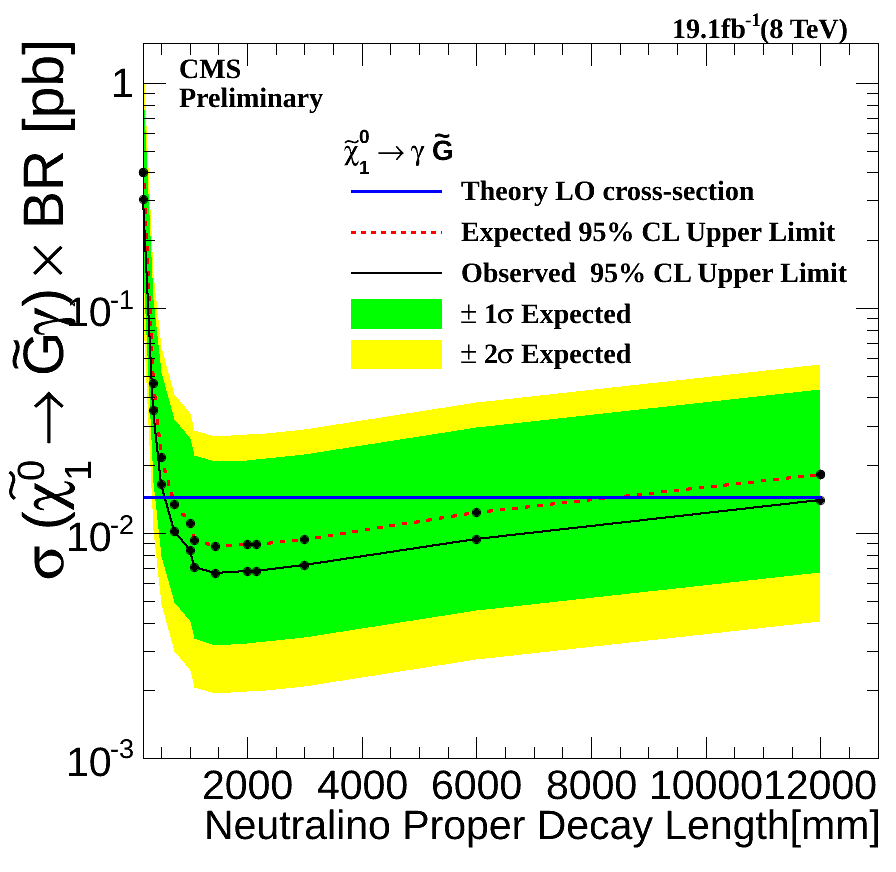
\includegraphics[height=5.5cm,width=5cm]{/home/tensr/Documents/TEN-HEP-PHD-THESIS/PHD_THESIS/PHD/THESISPLOTS/Neutralino_CrossSecTimesBR_Uplimit_HybridNew.png}
%}
\caption{HYBRIDNEW}
\label{fig:SUSY UL}
\end{minipage}
 \hspace{0.1cm}
 \begin{minipage}[b]{0.45\linewidth}
%\mbox{
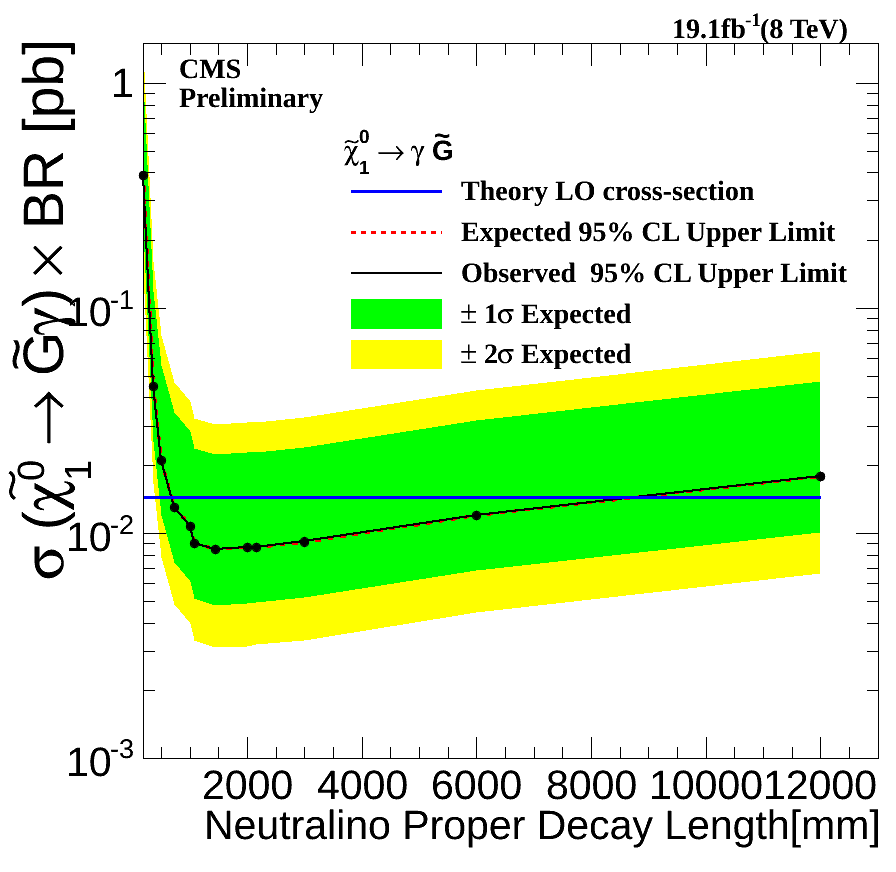
\includegraphics[height=5.5cm,width=5cm]{/home/tensr/Documents/TEN-HEP-PHD-THESIS/PHD_THESIS/PHD/THESISPLOTS/Neutralino_CrossSecTimesBR_Uplimit.png}
%}
%\caption{>= 1 Jets Upper Limit $\chi^{0}_{1}$ Decay}
\caption{ASYMTOTICS}
\label{fig:SUSY UL}
 \end{minipage}
\end{figure}
\end{frame}

\end{document}